\section{Node Flipping}

The Zhang and Shasha edit distance algorithm is specifically given for ordered trees, that is, the order of child nodes is taken to be significant. In attack trees without sequential conjunction, the order of nodes is not given to be significant~\cite{mauw_foundations_2006,jhawar_attack_2015}. This results in an issue where trees with identical, but unordered nodes are given to have a high edit distance. This is shown in Figure~\ref{fig:nodeflipping}, where two trees with identical information but different node order are given to have a distance of 2. This is due to the fact that the Zhang and Shasha algorithm is not designed to handle unordered trees. Zhang and Jiang have shown that the tree edit distance problem for unordered trees is an MAX SNP-hard~\cite{zhangMAXSNPhardResults1994}. We suggest a novel method for handling tree edit distance in unordered attack trees by taking advantage of the inherent structure of attack trees.


\begin{figure}
    \begin{subfigure}{.45\linewidth}
        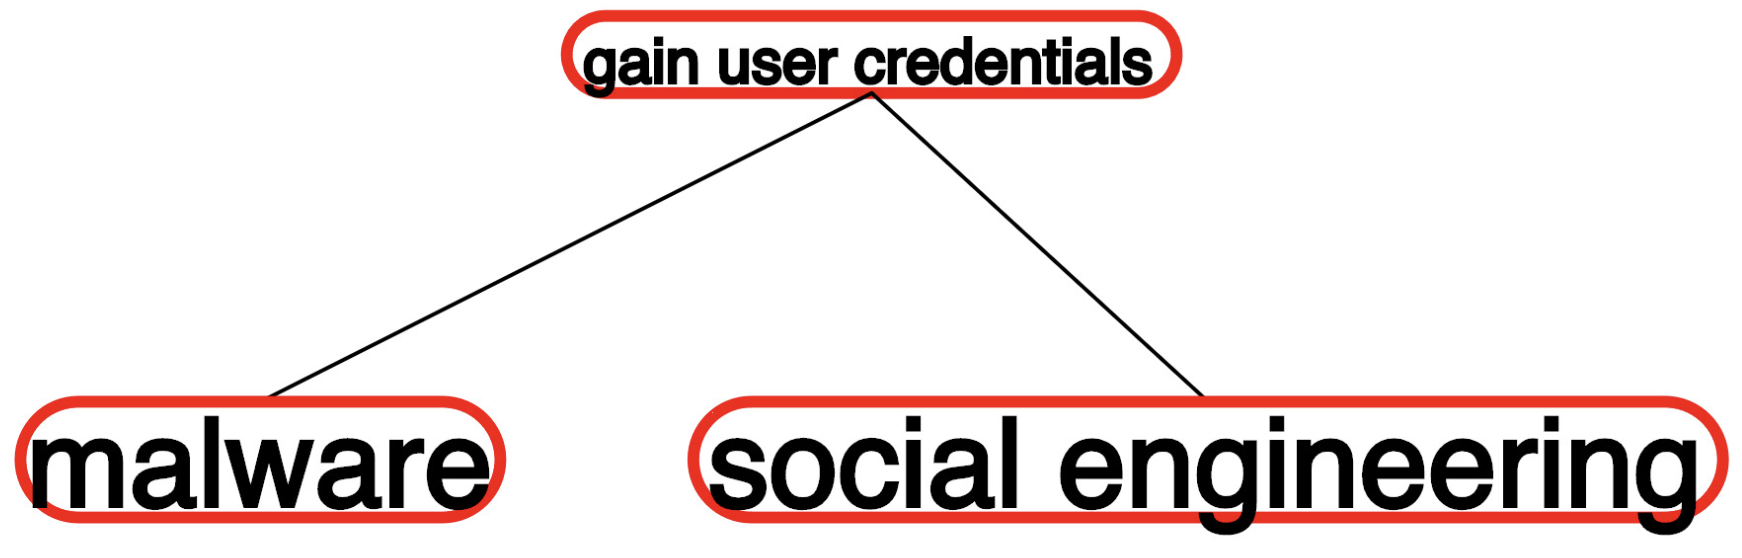
\includegraphics[width=\linewidth]{img/NodeFlip1.png}
    \end{subfigure}
    \begin{subfigure}{.45\linewidth}
        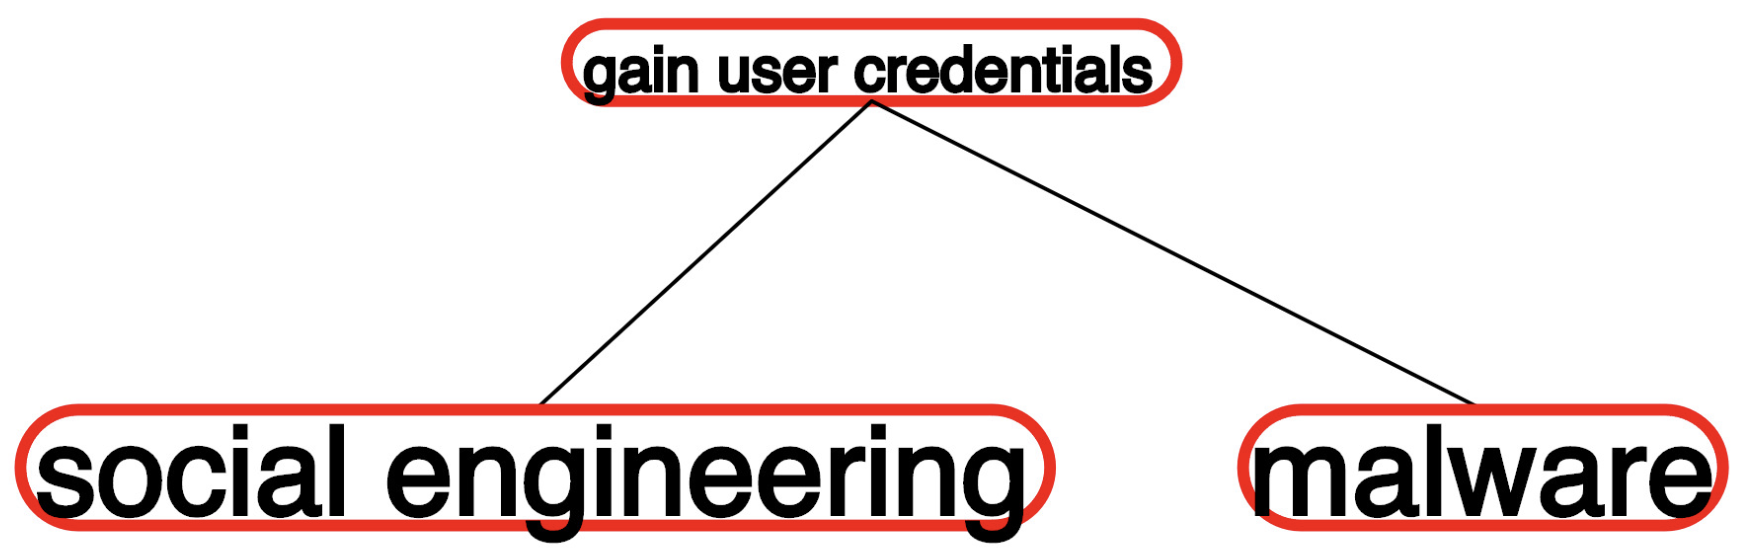
\includegraphics[width=\linewidth]{img/NodeFlip2.png}
    \end{subfigure}
    \caption{Two attack trees (subtrees of the example in Figure~\ref{fig:tartgetAT}) with identical information but different node order. These trees would evaluate to have a distance of 2 (two replacement operations).}
    \label{fig:nodeflipping}
\end{figure}

Attack trees, by virtue of their construction, tend to be organized in levels of abstraction. That is, with each new level of an attack tree, the nodes are given to be more specific than the nodes in the previous level. This is shown in Figure~\ref{fig:tartgetAT}, where the root node is given to be the most abstract (as the overall goal), while the leaf nodes are the most concrete (as the individual actions). From this, we find siblings in an attack tree to be on the same level of abstraction. As such, the order of siblings can be changed without affecting the meaning of the attack tree. By checking the order of sibling sets between the two attack trees




\subsection{Semantic mapping}

% Prior to calculation, a mapping is made between all nodes with the same labels, and this mapping is used to determine equivalence of nodes within the two trees. The labels of these nodes are typically given to be capital letters of the alphabet. However, in practical application, node labels are typically significantly more complex than mere letters.

% We introduce a new mapping step. As attack trees without sequential conjunction (\SAND\ refinements) are generally given to be unordered, we must implement an unordered semantic mapping. As described by Paa{\ss}en builds upon the work Zhang~\etal\ described for

% The steps:
% \begin{enumerate}
%     \item determine semantic cut off value $\epsilon$
%     \item list all node labels between both trees
%     \item calculate the semantic similarity between all node labels between the two trees
%           \begin{itemize}
%               \item this is given by comparing semantic embeddings
%               \item This is a value between 0 and 1, with 0 being no semantic similarity and 1 being identical semantic similarity
%           \end{itemize}
%     \item starting with node labels with the highest semantic similarity
%     \item remove these labels from both lists
%     \item repeat until at least one list is empty, or all semantic similarity values are below $\epsilon$
% \item Once we have our mappings, we reorder siblings as best as possible
% \begin{enumerate}
%     \item Starting with leaves, siblings can be swapped for no cost
%     \item Done if it improves the mapping
%     \item \textit{may result in local minima issues - but will be optimal enough}
% \end{enumerate}
% \end{enumerate}

\subsection{Semantic Sibling Reordering}
\begin{algorithm}
    \caption{An algorithm to reorder siblings based on semantic similarity}
    \label{alg:sibling_reorder}
    \begin{algorithmic}
        \State Two attack trees $T_1$ and $T_2$ according to Definition~\ref{def:attack-tree} with $a$ and $b$ total nodes respectively
        \State $M$ is the mapping of nodes between $T_1$ and $T_2$ \Comment{We give $m[0]$ and $m[1]$ to be the source and target nodes of a mapping for $m \in M$}
        \State $M \gets T_1[a]\mapsto T_2[b]$\Comment{Root nodes are always mapped}
        \For{$m \in M$}

        \State $D \gets []$ \Comment{Matrix of semantic similarity values}
        \For{left-wise index $i$ in $m[0].\text{children}$}
            \For{leftwise index $j$ in $m[1].\text{children}$}
                \State $D[i][j] \gets \delta(m[0].\text{children}[i].\text{label}, m[1].\text{children}[j].\text{label})$
            \EndFor
        \EndFor
        \State $M_t \gets \emptyset$ \Comment{Temporary set of mappings} 
        \While{$D$ is not empty}
            \State $i, j \gets \text{argmax}(D)$ \Comment{Largest value in $D$}
            \State $M_t \gets M_t \cup m[0].\text{children}[i]\mapsto m[1].\text{children}[j]$
            \State $D \gets D - i$ \Comment{Remove row $i$}
            \State $D \gets D - j$ \Comment{Remove column $j$}
        \EndWhile
        \For{$p$ in $M_t$}
            \If{indicies $i$, $j$ of $p$ are not equal}
                \State{Swap nodes $i$ and $j$ \textbf{in $T_1$}}
            \EndIf
        \EndFor
        \State $M \gets M \cup M_t$
        \EndFor
    \end{algorithmic}
    \end{algorithm}